\documentclass[12pt]{article}
\usepackage{mathrsfs}
\usepackage{amsmath}
\usepackage{amsthm}
\usepackage[center]{caption}
\usepackage{cite}
\usepackage{picinpar}
\usepackage{bbm}
\usepackage{subfloat}
\usepackage{subfigure}
\usepackage{fancyhdr,graphicx}
\usepackage{amsfonts}
\usepackage{amssymb}
\usepackage{latexsym,bm}
\usepackage{newlfont}

\textwidth 165 mm \textheight 250 mm \hoffset -1.5cm \voffset-2.5cm
%%theorem enviroment--------------------------------------------

\newtheorem{thm}{Theorem}[section]
\newtheorem{lemma}[thm]{Lemma}
\newtheorem{cor}[thm]{Corollary}
\newtheorem{pro}[thm]{Proposition}
\newtheorem{defn}[thm]{Definition}
\newtheorem{claim}[thm]{Claim}
\newtheorem{remark}[thm]{Remark}
\newcommand{\pf}{\vspace{-1mm}\noindent{{\em Proof.}\, }}

%%%%%%%%%%%%%%%%%%%%%
%����fig
\renewcommand\figurename{Figure}
\makeatletter
\long\def\@makecaption#1#2{%
 \vskip\abovecaptionskip
  \sbox\@tempboxa{{#1.}\quad #2}%
 \ifdim \wd\@tempboxa >\hsize
    { #1.}\quad #2\par
     \else
  \global \@minipagefalse
   \hb@xt@\hsize{\hfil\box\@tempboxa\hfil}%
   \fi
   \vskip\belowcaptionskip}
\makeatother

%%%%%%%%%%%%%
\renewcommand{\baselinestretch}{1.2}

\setlength{\baselineskip}{17pt}

%%article-------------------------------------------------------

\title{\bf{$l_1$-embeddability of small irreducible quadrilateral  M\"{o}bius maps}\thanks{This project is
 supported by NSFC (Grant Nos $11861032$ and $11501282$) and the Natural Science Foundation of ShanDong Province (ZR2018MA010). }}

\author{Guangfu Wang$^{1}$, Sergey Shpectorov$^2$, Jianxin Wei$^{3}$\\
\small{1. School of Science, East China Jiaotong University,
Nanchang, 330013, China.}\\
\small{2. School of Mathematics, University of Birmingham,
Edgbaston, Birmingham, B15 2TT, UK. } \\
 \small{3. School of Mathematics and Statistics Science, Ludong University, Yantai, Shandong 264025,  China.}\\
\small{E-mail addresses: gfwang@ecjtu.edu.cn, s.shpectorov@bham.ac.uk, wjx0426@163.com.} }
\date{}

%%--------------------------------------------------------------
\begin{document}

\maketitle

\makeatletter
\newcommand{\rmnum}[1]{\romannumeral #1} ����
\newcommand{\Rmnum}[1]{\expandafter\@slowromancap\romannumeral #1@}
\makeatother


\begin{abstract}



A graph is   an  {\it $l_1$-graph}  if its vertices can be labeled
by binary vectors in such a way that the Hamming distance between
the binary addresses is, up to scale, the distance in the graph
between the corresponding vertices. A small irreducible
quadrilateral M\"{o}bius map $(M, \Gamma)$ is a class of
quadrilateral   M\"{o}bius map with girth $3$ which does not
contain a proper M\"{o}bius submap. In
this article, we determine among these maps which are
$l_1$-embeddable.

\noindent \textbf{Key words:}\quad $l_1$-embeddable; irreducible;
quadrilateral M\"{o}bius map

\end{abstract}

%%introduction--------------------------------------------------


\section{Introduction}
\setlength{\unitlength}{1cm} \setlength{\unitlength}{1cm}



As a subsequent result of \cite{Wan16}, to make this article self-contained, we introduce some necessary terminologies.
For  graphs $G$ and $H$,  and a given positive integer $\lambda$, a mapping
$\phi: V(G)\rightarrow V(H)$, is called a $\lambda$-{\em embedding}
  if, for any two vertices $x, y$
of $G$, we have $d_H(\phi(x), \phi(y))=\lambda d_{G}(x,y).$ If
$\lambda=1$, then $\phi$ is called an {\em isometric embedding} of
$G$ into $H$.

 An \textit{$n$-dimensional hypercube} $Q_n$ is constructed as
follows:
 Let $\Omega=\{1,2,\ldots, n\}$. The vertices of $Q_n$ are all subsets of $\Omega$.
 Two vertices $A$ and $B$ are adjacent if and only if  $|A\triangle B|=1$,
 where $\triangle$ denotes the symmetric difference of sets,
  i.e., $A\triangle B=(A\setminus B)\cup (B\setminus A)$.
  Then the distance between any two vertices $A$ and $B$ in $Q_n$
  is equal to $|A\triangle B|$.

A connected graph $G$ is
called an {\em $l_1$-graph} if there is a distance-preserving
embedding $\varphi$ into some $\mathbb{R}^n$ equipped with the
1-norm $\parallel\cdot\parallel_1$, that is,
$d_G(x,y)=\|\varphi(x)-\varphi(y)\|_1$ for all vertices $x, y$ of
$G$. Recall that, for $x=(x_1, x_2,\ldots,x_n)\in \mathbb{R}^n$, we
have $\|x\|_1=\sum\limits_{i=1}^n|x_i|$.

 Assouad and Deza
\cite{Ass80} showed that a graph $G$ is an $l_1$-graph if and only
if it admits a $\lambda$-embedding into a cube $Q_k$ for some
integers $\lambda$ and $k$. If $\lambda=1$, $G$ is also called a
\textit{partial cube}.

  A \textit{map} is an ordered pair
$(K,G)$, where $K$ is a compact
surface (possibly with boundary) and $G$ is a graph regularly
embedded in $K$, such that:
\begin{enumerate}
\item each connected component of $K\setminus G$ is homeomorphic to an open disk;
\item the boundary of $K$ is a subgraph of $G$.
\end{enumerate}

 Note that,
by definition, a map can be disconnected. A \textit{face }of $(K,G)$
is the closure in $K$ of a connected component of $K\setminus G$. A
face with $k$ edges will be called a $k$\textit{-gon}. If $K$ has a
boundary, a face containing at least one boundary vertex is called a
\textit{boundary face}. Faces containing no boundary vertices are
called \textit{inner faces}. An edge incident with just one face is
called a  {\em boundary edge}. Other edges are called {\em inner
edges}. A map $(K,G)$ is called a \textit{quadrilateral map} if each
face of $(K,G)$ is a $4$-gon and, all of its inner vertices are
4-valent and
 all of boundary vertices are 2-, 3-, or 4-valent.  If $K$ is  a disk, $(K,G)$ is called a
 \textit{quadrilateral plane map}.
(See Figure \ref{PG}.)   If $K$  is   a M\"{o}bius
strip, $(K, G)$ is called a
\textit{quadrilateral M\"{o}bius map}.
(See Figure \ref{MQ}.)
  Additionally, we are requiring certain nondegeneration of the map
  around each of its vertices. The easiest way
to explain these  restrictions is that all possible
configurations of faces incident with a vertex $v$ must be as
shown in Figure \ref{neighbors}, where the shaded parts are faces.
The vertex $v$ is boundary  in cases $(a)$-$(c)$ and it is inner in
$(d)$.
The other terminations not introduced here can  refer to \cite{Wan16}.




\begin{figure}[!htbp]
  \centering
  \begin{minipage}[c]{0.5\textwidth}
    \centering
    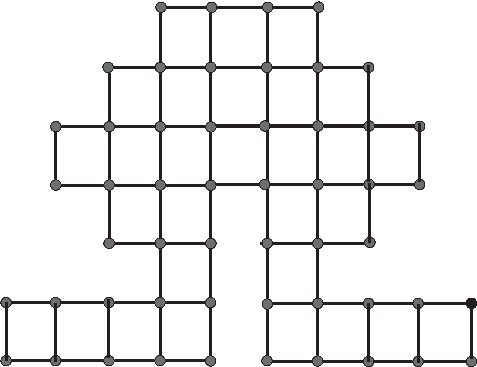
\includegraphics[totalheight=3.5cm]{PG}
    \caption{\label{PG}A quadrilateral plane map.}
  \end{minipage}%
  \hspace{2em}
  \begin{minipage}[c]{0.4\textwidth}
    \centering
    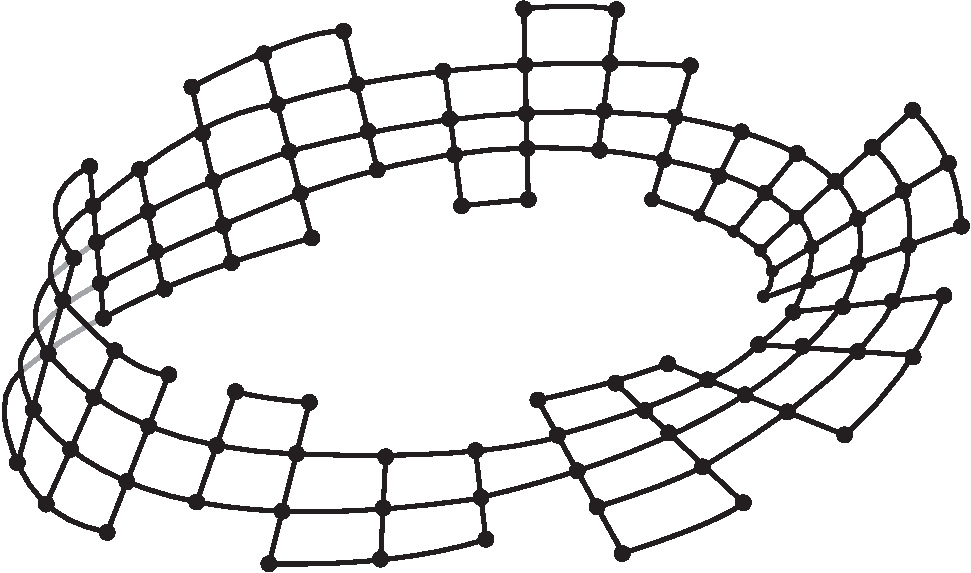
\includegraphics[totalheight=3.5cm]{MQ2}
  \caption{\label{MQ} A quadrilateral  M\"{o}bius map. }
   \end{minipage}
\end{figure}

\begin{figure}[!htbp]
         \centering
           \subfigure[2-valent]{\label{2nei}
           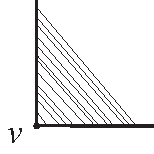
\includegraphics[totalheight=1.8cm]{2val}}\hspace{1cm}
           \subfigure[3-valent]{\label{3nei}
           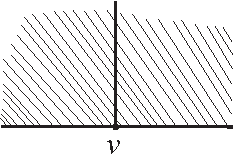
\includegraphics[totalheight=2cm]{3val}}\hspace{1cm}
           \subfigure[4-valent]{\label{4nei}
           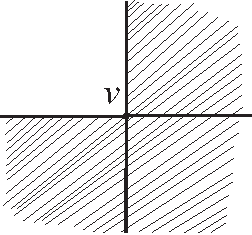
\includegraphics[totalheight=2.4cm]{4val-1}}\hspace{1cm}
            \subfigure[4-valent]{\label{4neb}
           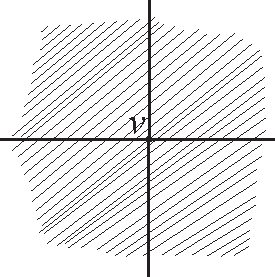
\includegraphics[totalheight=2.4cm]{4val}}
             \caption{\label{neighbors}All possible faces incident with a vertex $v$.}
\end{figure}


A quadrilateral M\"{o}bius map $(M,\Gamma)$ is called
\textit{irreducible} if it does not contain a proper M\"{o}bius map.
We call a quadrilateral M\"{o}bius map $(M, \Gamma)$
\textit{generic}
if all faces of $(M, \Gamma)$  are isometric. Otherwise, call it  \textit{small}.
In this article, we study the $l_1$-embeddability of
small irreducible quadrilateral M\"{o}bius maps. The
$l_1$-embeddability of generic quadrilateral M\"{o}bius maps is
refer to \cite{Wan16}.



\section{Fundamentals}
First we
introduce an important necessary condition of $l_1$-graphs.

\begin{lemma}\cite{Tyl60}\label{5gon}
If $G$ is an $l_1$-graph then $d_G$ must satisfy the following
$5$-gonal inequality: for any five vertices $x,y,a,b,c$ of $G$,
$$d(x,y)+(d(a,b)+d(b,c)+d(a,c))\leq (d(x,a)+d(x,b)+d(x,c))+(d(y,a)+d(y,b)+d(y,c)).$$
\end{lemma}

Avis \cite{Avi81}  showed that  a bipartite graph $G$ is a partial
cube if and only if $d_G$ satisfies the 5-gonal inequality.

Above all, there is a forbidden subgraph in any $l_1$-embeddable graph which is important to
us. See the graph $G_1$ in Figure \ref{G1}.
\begin{figure}[!htbp]
\centering
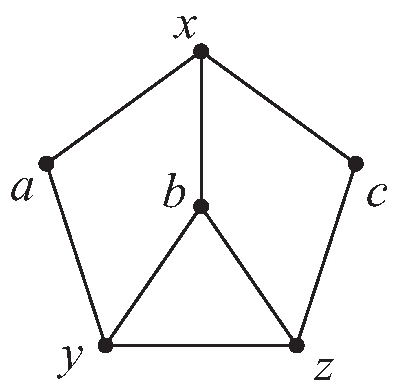
\includegraphics[width=3.5cm]{G1}
\caption{$G_1$\label{G1}}
\end{figure}

\begin{lemma}
The graph $G_1$ from Figure \ref{G1} is not $l_1$-embeddable.
\end{lemma}
\begin{proof}
For the vertices $x,y,a,b$ and $c$, $d(a,b)+d(b,c)+d(a,c)+d(x,y)$=8,
but
$$(d(x,a)+d(x,b)+d(x,c))+(d(y,a)+d(y,b)+d(y,c))=7.$$  That indicates that  $x,y,a,b$ and $c$
violate the 5-gonal inequality.
\end{proof}


\begin{figure}[!htbp]
          \centering
           \subfigure[\label{k4}$K_4$.]{
           \includegraphics[totalheight=3cm]{K4}}\hspace{1cm}
           \subfigure[\label{W5-e}$W_5-e$.]{
           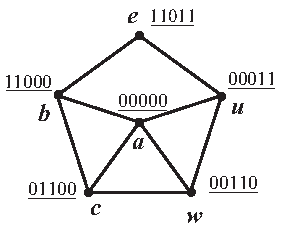
\includegraphics[totalheight=3cm]{W5-e}}\hspace{1cm}
           \subfigure[\label{Lambda}$\Lambda$.]{
           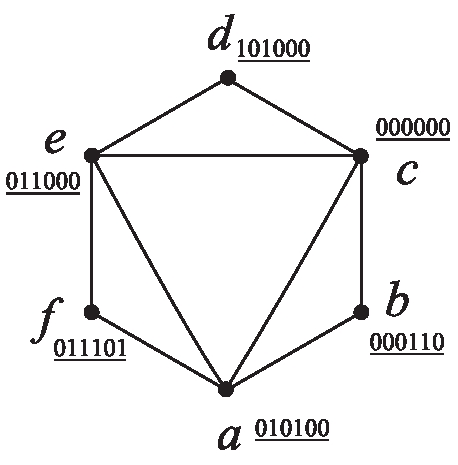
\includegraphics[totalheight=3.2cm]{Lambda}}
         \caption{Three special ~$l_1$-embeddable graphs.\label{three}}
\end{figure}


On the other hand, the three graphs in Figure \ref{three} are all
$l_1$-embeddable, as shown by the 0,1-sequences in Figure
\ref{three}. Namely, we can state the followings:

\begin{lemma}
\begin{enumerate}

\item  The complete graph $K_4$ is   scale-2-embeddable into $Q_4$.

\item The graph $W_5-e$ is   scale-2-embeddable into
$Q_5$.

\item The Graph $\Lambda$ is   scale-2-embeddable into
$Q_6$.\hfill $\square$
\end{enumerate}
\end{lemma}

\begin{defn}
The Euler characteristic of a map $(K,G)$, denoted by $\chi(G)$,
is the Euler characteristic of the surface $K$, which is
obtained by summing the number of vertices and faces and
subtracting the number of edges.
\end{defn}

From  \cite{Gro87}, we know, when $K$ is closed, that
$\chi(G)=2-2g$ if $K$ is orientable with $g$ handles (Theorem
3.3.1 \cite{Gro87}) and $\chi(G)=2-k$ if $K$ is non-orientable
obtained by attaching $k$ crosscaps to a sphere(Theorem 3.3.2
\cite{Gro87}). As we know that, when $K$ is a disk, cylinder, or M\"{o}bius strip,
$\chi(G)=1$, $0$, or $0$, respectively. Conversely, if $(K,G)$
is connected and $\chi(G)$ is $1$, or $0$, then $(K,G)$ is
either a plane map, or a cylinder map, or a M\"{o}bius map. If
$(K,G)$ is disconnected then $\chi(G)$ is the sum of the Euler
characteristics of its components.

For any quadrilateral map $(K, G)$, let $n_2$ and $n_4$ denote
the number of boundary vertices of valency 2 and 4, respectively. We
call $b(G):=n_2-n_4$ the \textit{balance} of $(K,G)$.

By the Euler characteristic of a map,  Wang and   Shpectorov showed that

\begin{lemma}\label{bal}\cite{Wan16}
 \[b(G)=\left\{
 \begin{array}{rl}
               4,    &\mbox{if $K$ is a disk,}\\
               0,    &\mbox{if $K$ is a cylinder or   M\"{o}bius strip.}
 \end{array}
 \right.
 \]
\hfill$\square$
 \end{lemma}


\section{Labels of $l_1$-graphs}

We introduce  labels on $l_1$-graphs introduced  in \cite{Shp93} and
later used in \cite{Dez96,Dez09,Dez05,Mar07}.



Let $G$ be a finite $l_1$-graph and $\phi$ be a scale $\lambda$
embedding of $G$ in $Q_n$. We assign to each edge $uv$ of $G$ a
\textit{label} $l(uv)$ as follows: $l(uv)=\phi(u)\triangle \phi(v)$.
For each edge $e=uv$ of $G$, $|\phi(u)\triangle
\phi(v)|=d_{Q_n}(\phi(u),\phi(v))=\lambda\cdot d_G(u,v)=\lambda$.
That is, every edge label consists of precisely $\lambda$ elements
from \{1,2,\ldots, $n$\}.

A subgraph $H$ of $G$ is called \textit{isometric} if
$d_H(u,v)=d_G(u,v)$ for any vertices $u,v$ of $H$. Generally, let
$C_k=v_0v_1 \ldots v_{k-1}v_0$ be a cycle. By an isometric cycle in
$G$, we mean the image in $G$ of an isometric embedding $C_k$ into
$G$, for any $k$. Two edges $v_iv_{i+1}$ and $v_jv_{j+1}$  of $C_k$
with $0\leq i, j\leq k-1$ are \textit{opposite} if
$d_{C_k}(v_i,v_j)=d_{C_k}(v_{i+1},v_{j+1})$ and equal to the
diameter of $C_k$, where $v_{k}=v_0$. Thus, every edge has a unique
opposite edge if $k$ is even; and has two opposite edges, otherwise.

\begin{lemma}\cite{Dez96,Mar07}\label{isocycle}
Suppose that $C_k$ is an isometric cycle of $G$ and $uv$ and $xy$
are a pair of opposite edges of $C_k$. If $k$ is even, then
$l(uv)=l(xy)$, while if $k$ is odd, then $|l(xy)\cap
l(uv)|=\frac{\lambda}{2}$. Furthermore if $k$ is odd and $vw$ is the
second edge opposite to $xy$ then $l(xy)\subset l(uv)\cup l(vw)$.
The labels of non-opposite edges are disjoint.\hfill $\square$
\end{lemma}

\begin{lemma} \cite{Wan11}\label{labelneq}
If a simple graph $G$  is an $l_1$-graph, then the labels on
adjacent edges of $G$ are never equal.\hfill $\square$
\end{lemma}



\section{Main result}
Suppose that $(M,\Gamma)$ is a small  quadrilateral  M\"{o}bius map.  Then some face of $\Gamma$ is not isometric,
and $\Gamma$ has a 3-cycle $C$. If
$C$ is nulhomotopic, then the region bounded by $C$ form a quadrilateral plane
map.    According  to Lemma \ref{bal},  it must contain at least  four $2$-valent boundary vertices, but the boundary $C$ has just three 2-valent boundary vertices, a contradiction.
Hence $C$ is a non-nulhomotopic cycle. Throughout this section we assume that
$(M,\Gamma)$ is a small  $l_1$-embeddable  quadrilateral  M\"{o}bius
map.

First of all,  we consider a $3$-cycle $C$ of $(M,\Gamma)$.



\begin{lemma}\label{bound}
Some, but not all edges of $C$ are inner.
\end{lemma}
\begin{proof}
 If all edges of $C$ are inner, after cutting along $C$ we obtain one or
more maps with the total of 3 pieces of boundary and the total
characteristic of 0. Let $C_1$ and $C_2$ be the two
cycles corresponding to $C$. If one piece is a plane map, it has the
boundary consisting of edges of $C_1$ or $C_2$. It is impossible,
since $C$ is non-nulhomotopic. So the characteristic of every map is
0.
 Therefore, we can only
have two maps, one ($M_1,\Gamma_1$) on a cylinder (accounting for
two pieces of boundary $B$ and $C_1$, say) and the other ($M_2,
\Gamma_2$) on a M\"{o}bius band with boundary $C_2$.  We focus on
$(M_2,\Gamma_2)$. Let $m_2$ and $f_2$ be the numbers of  edges and faces of $(M_2,\Gamma_2)$, respectively.
Then, we have $4f_2+3=2m_2$. This is impossible.

If all edges of $C$  are boundary, then $C$ is the boundary of  $(M,\Gamma)$.   Let $m$ and $f$ be the numbers of  edges and faces of $(M,\Gamma)$, respectively. We have $4f+3=2m$, a contradiction.  This completes the lemma.
\end{proof}

\begin{lemma}\label{1inner}
The cycle $C$  has exactly one inner edge.
\end{lemma}
\begin{proof}
Suppose that $C=abc$ has two inner edges, say $bc,ca$.By Lemma \ref{bound}, $ab$ is a boundary edge. Hence $b$ is a boundary vertex, and $c$ is surrounded by four faces. By the construction of the M\"{o}bius map, we know that there are two cases to consider:

Case 1. $ab$ and $bc$ are incident with different faces. (See Figure \ref{differface}.)
\begin{figure}[!htbp]
\centering
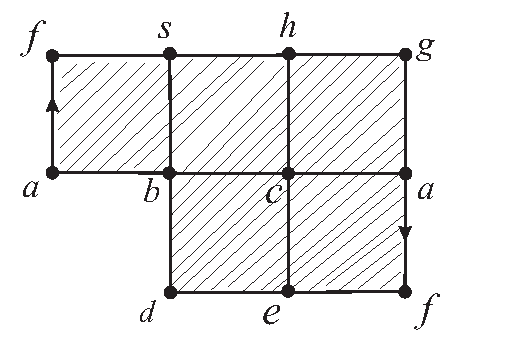
\includegraphics[totalheight=3cm]{two-inner-edge}
\caption{\label{differface}$C$ has two inner edges $bc$ and $ca$, and $ab$ and $bc$ are incident with different faces.}
\end{figure}

Since $G$ is $l_1$-embeddable and  the faces $absf, afec, cedb$ are isometric 4-cycles, by Lemma \ref{isocycle},   $l(af)=l(bs)$ and $l(af)=l(ce)=l(bd)$. Therefore $l(bs)=l(bd)$, a contradiction to Lemma \ref{labelneq}.

Case 2. $ab$ and $bc$ are incident with  a same  face. (See Figure \ref{twoinner}.)

\begin{figure}[!htbp]
          \centering
           \subfigure[\label{twoinner}]{
           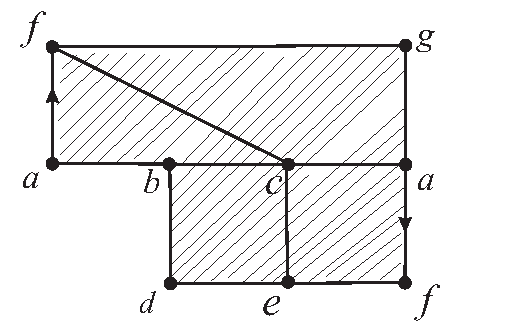
\includegraphics[totalheight=3cm]{two-inner-edge2}}\hspace{1cm}
           \subfigure[\label{twoinner2}]{
           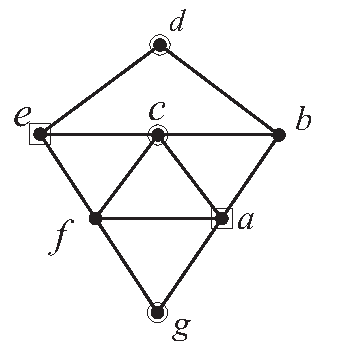
\includegraphics[totalheight=3.4cm]{two-inner-edge3}}\hspace{1cm}
           \caption{}
\end{figure}


In fact, the graph in figure \ref{twoinner} is isomorphic to the graph in figure \ref{twoinner2}. But the graph in  figure \ref{twoinner2} is not $l_1$-embeddable, since the five vertices $a,e, d,c,g$ violate the 5-gonal inequality. In fact,
\begin{equation*}
\begin{split}
&d(e,a)+d(d,c)+d(c,g)+d(d,g)\\
&=2+2+2+3=9\\
&>(d(e,d)+d(e,c)+d(e,g)+d(a,d)+d(a,c)+d(a,g))\\
&=(1+1+2)+(2+1+1)\\
&=8.
\end{split}
\end{equation*}

To sum up, $C$ cannot have two inner edges, so $C$ has only one inner edge.
\end{proof}


\begin{lemma}\label{twoedges}
Two edges of  $C$ bound one face of $(M,\Gamma)$.
\end{lemma}
\begin{proof}
Suppose that no two edges of $C=abc$ bound a face. That is, the  three edges of $C$ are  incident with distinct faces.  From Lemma \ref{1inner}, let  $ac$ be the inner edge
 shared by  $cagh$ and $acef$ (see Figure \ref{noaface}).  Then we know that  $l(ce)=l(af)=l(bd)=l(hc)$, a contradiction to Lemma \ref{labelneq}.
\begin{figure}[!htbp]
\centering
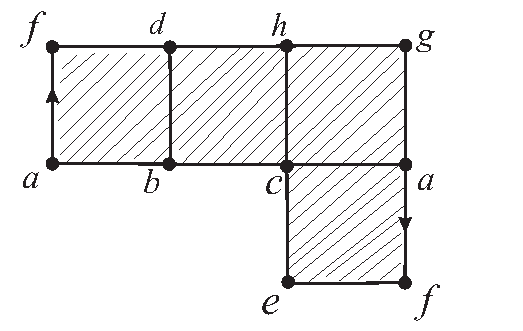
\includegraphics[totalheight=3cm]{boundoneface}
\caption{\label{noaface}Three edges of $C$ are  incident with distinct faces.  $ac$ is the inner edge
 shared by  $cagh$ and $acef$.\label{acinner}}
\end{figure}
\end{proof}



\begin{thm}
Let $(M,\Gamma)$ be a small irreducible quadrilateral M\"{o}bius map. If $(M,\Gamma)$ is $l_1$-embeddable, then $\Gamma$
is isomorphic to one of the following graphs: $K_4$, $W_5-e$ or
$\Lambda$.
\end{thm}

\begin{proof}
Suppose $C=abc$ is a $3$-cycle of $(M,\Gamma)$.
By Lemma \ref{1inner}, $C$ has only one inner edge, say $ac$.

\textbf{Case 1.} $ac$ and $ab$ are incident with a same face. Suppose $ac$
is shared by two faces $abdc$ and $afec$. (See Figure \ref{acinner}.)

\begin{figure}[!htbp]
\centering
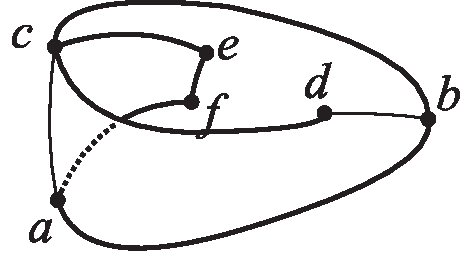
\includegraphics[totalheight=2.5cm]{acinner}
\caption{$ac$ is
 shared by  $abdc$ and $afec$.\label{acinner}}
\end{figure}

\begin{enumerate}
\item   $e=b$.

\begin{enumerate}
\item If $f=d$, the graph $\Gamma$ is
isomorphic to
$K_4$. (See Figure \ref{K42}.)
\begin{figure}[!htbp]
\centering
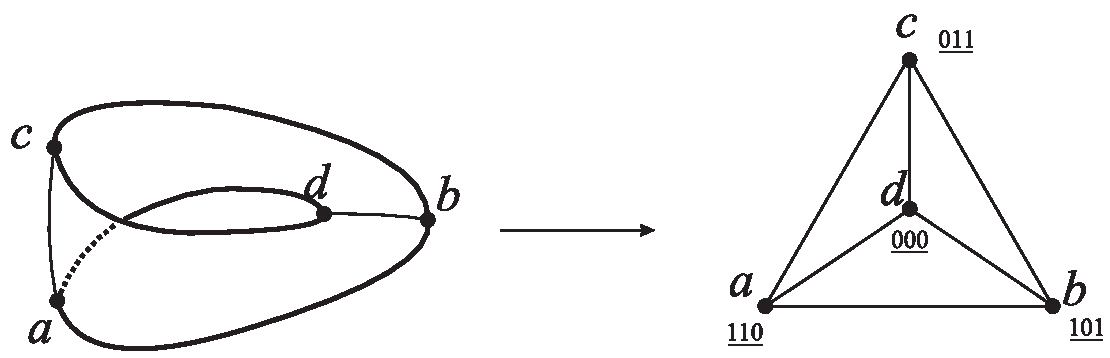
\includegraphics[totalheight=3cm]{k42}
\caption{$e=b, f=d.$\label{K42}}
\end{figure}


\item If $f\neq d$, $b$ has 4 neighbors $c,f,d$ and $a$. Since $bc$ and $ab$ are
 boundary, $bf$ and $bd$ bound a face $f_3=bdgf$. Then the graph
 $\Gamma$ is isomorphic to $W_5-e$. Hence the map is $l_1$-embeddable. (See Figure \ref{W5-e2}.)
\begin{figure}[!htbp]
\centering
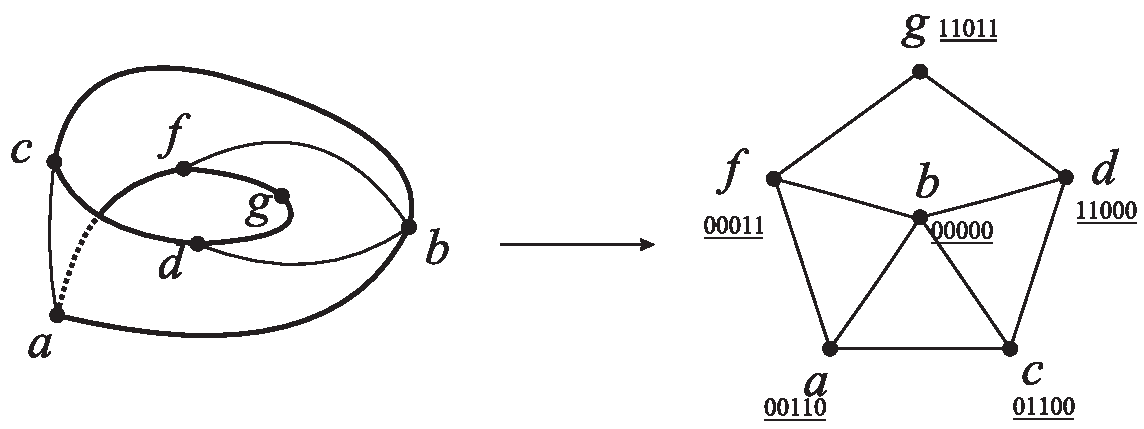
\includegraphics[totalheight=3.5cm]{W5-e2}
\caption{$e=b, f\neq d$\label{W5-e2}}
\end{figure}

\end{enumerate}
\item $e\neq b$.

\begin{enumerate}
\item If $f=d$, then $abd$ is a 3-cycle. So $abd$ is a non-nulhomotopic cycle and $adbc$ is nulhomotopic.
Therefore, the region bounded by $adbc$ is a quadrilateral plane map. (See Figure \ref{bfd}.) By Lemma \ref{bal}, this plane map has
at least four 2-valent boundary vertices. While $c$ and $d$ are not 2-valent, this plane map has at most two
2-valent boundary vertices, a contradiction.
\begin{figure}[!htbp]
\centering
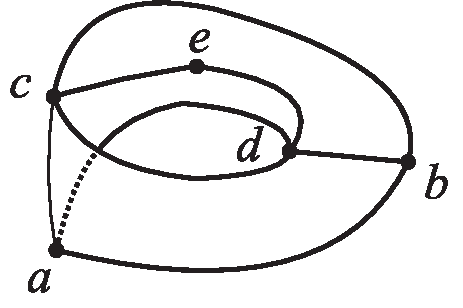
\includegraphics[width=3.5cm]{fd}
\caption{$e\neq b, f=d$\label{bfd}}
\end{figure}


\item If $f\neq d$, Since $bc$ is boundary and $c$ is 4-valent, let $cegb$ be a face incident with $bc$ and $ce$.

\begin{enumerate}
\item If $g=d$, then this map is a quadrilateral M\"{o}bius map. It
is isomorphic to $W_5-e$. (See Figure \ref{w5e3}.)
\begin{figure}[!htbp]
\centering
\includegraphics[totalheight=3.5cm]{w5-e3}
\caption{$e\neq b, f\neq d, g=d.$\label{w5e3}}
\end{figure}

\item If $g\neq d$, then $b$ has 4 neighbors $c,g, d$ and $a$. Since
$bc$ and $ba$ are boundary, $gb$ and $bd$ bound a face $gbdh$.  This
is a quadrilateral M\"{o}bius map. But the graph induced by the vertices
$a$, $b$, $c$, $e$, $f$
$g$ is isomorphic to the graph $G_1$. It is also an isometric
submap in $\Gamma$. By Lemma \ref{G1}, $G_1$ is not
$l_1$-embeddable.  So $\Gamma$ is not $l_1$-embeddable. (See Figure \ref{G11}.)

\begin{figure}[!htbp]
\centering
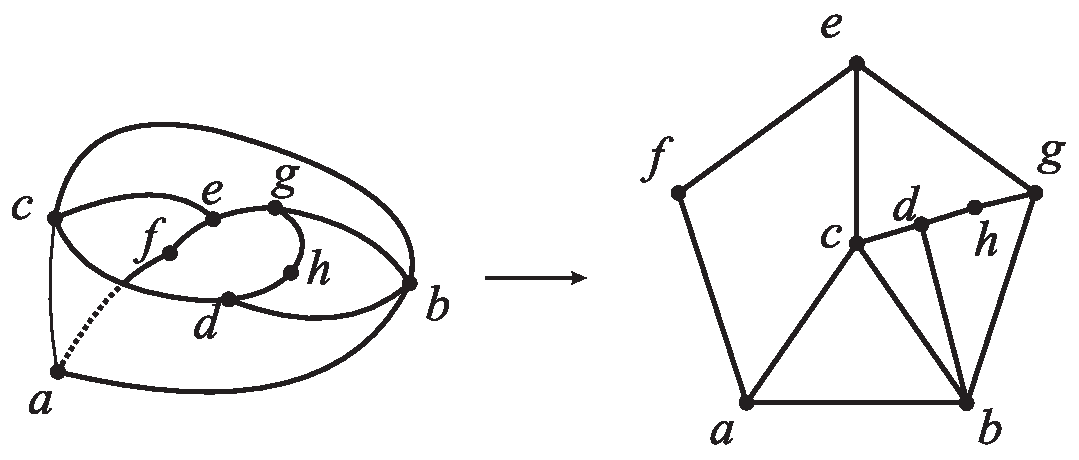
\includegraphics[totalheight=3cm]{G11}
\caption{$e\neq b, f\neq d, g\neq d.$\label{G11}}
\end{figure}


\end{enumerate}
\end{enumerate}
\end{enumerate}

\textbf{Case 2.} $ac$ and $ab$ are not incident with a same face.

Suppose that $ac$ is shared by $adgc$ and $afec$. Now $a$ is
4-valent. $ad$ and $ab$ bound a face.

 \begin{enumerate}
\item $d=e$. Then $abcd$ bound a face. This graph is isomorphic to
$\Lambda$. (See Figure \ref{lambda2}.)

\begin{figure}[!htbp]
\centering
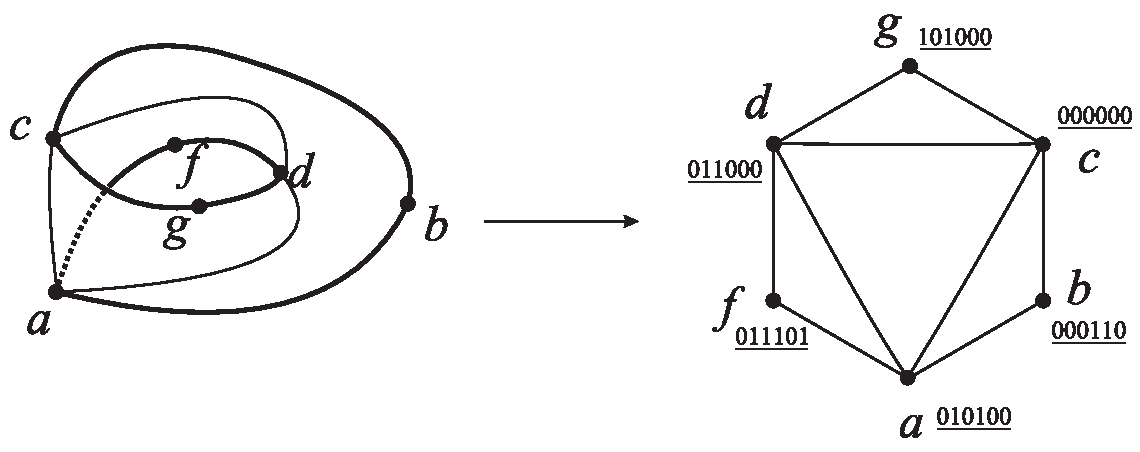
\includegraphics[totalheight=3cm]{lambda2}
\caption{$d=e.$\label{lambda2}}
\end{figure}

\item $d\neq e$. Suppose that $adhb$ is the face incident with $ad$
and $ab$.
\begin{enumerate}
\item If $h=g$, then $abgc$ is a 4-cycle which is nulhomotopic.
The region $R$ bounded by $abgc$
 is a quadrilateral plane map. By Lemma \ref{bal},
 $R$ has at least four 2-valent boundary vertices. But $a$ and $g$
 are not 2-valent, a contradiction. (See Figure \ref{hg}.)

 \begin{figure}[!htbp]
\centering
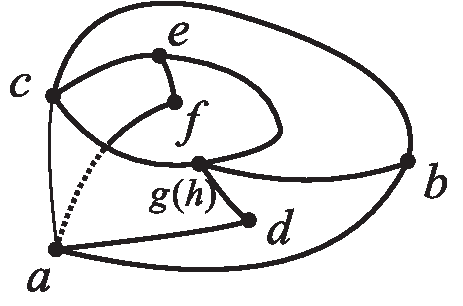
\includegraphics[totalheight=3cm]{hg}
\caption{$d\neq e, h=g.$\label{hg}}
\end{figure}


 \item  $h\neq g$. Let $bcei$ be the face bounded by $ce$ and $bc$.

 \begin{enumerate}

 \item If $i=h$ then this is a M\"{o}bius
 map $(M,\Gamma)$. The subgraph induced by $a$, $b$, $c$,
  $d$, $g$ and $h$ is isomorphic to the graph $G_1$. By Lemma
  \ref{G1}, $G_1$ is not $l_1$-embeddable. Therefore $(M,\Gamma)$
  is not $l_1$-embeddable. (See Figure \ref{ih}.)
\begin{figure}[!htbp]
\centering
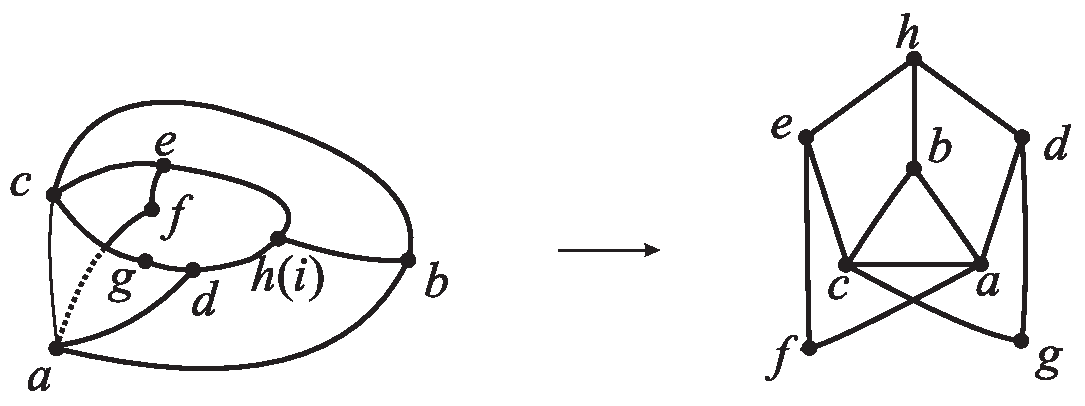
\includegraphics[totalheight=3cm]{ih}
\caption{$d\neq e, h\neq g, i=h.$\label{ih}}
\end{figure}



  \item If $i\neq h$, then $bi$ and $bh$ bound another face $bijh$.
  In this M\"{o}bius map, the subgraph $H$ induced by $a$, $b$, $c$,
  $d$, $g$ and $h$ is isomorphic to $G_1$, and it is not
  $l_1$-embeddable. Since $H$ is isometric in $(M,\Gamma)$,
  $(M,\Gamma)$ is not $l_1$-embeddable. (See Figure \ref{ineqh}.)

  \begin{figure}[!htbp]
\centering
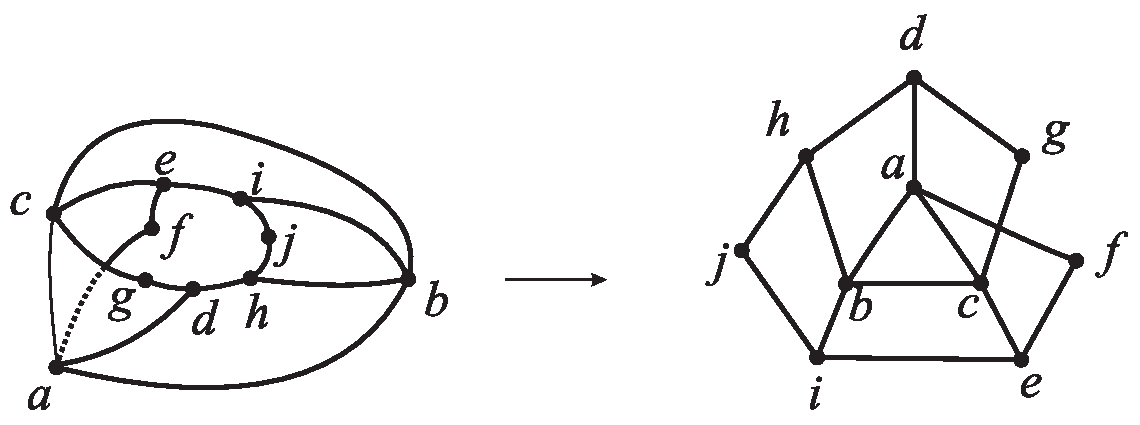
\includegraphics[totalheight=3cm]{ineqh}
\caption{$d\neq e, h\neq g, i\neq h.$\label{ineqh}}
\end{figure}
  \end{enumerate}
 \end{enumerate}
 \end{enumerate}

 To sum up, if $(M,\Gamma)$ is $l_1$-embeddable, it is isomorphic to $K_4$, $W_5-e$ or $\Lambda$.
\end{proof}


At the end of this article, we consider   reducible quadrilateral M\"{o}bius maps. First, we introduce a theorem of $l_1$-embeddability of graphs under edge-gluing operations.

\begin{thm}\cite{Wan13}\label{glueedge}
Let $G$ and $H$ be $l_1$-graphs. If at least one of them is bipartite, then the new graph $G\cup_e H$ by gluing $G$ and $H$ along an edge is  $l_1$-embeddable.
\end{thm}

We can obtain a reducible quadrilateral M\"{o}bius map from an irreducible quadrilateral M\"{o}bius map and a quadrilateral plane map by identifying an edge. By Theorem \ref{glueedge}, if we glue a quadrilateral plane map to the map in Figure \ref{K42}
at the edge $ad$, $ab$, $bc$ or $bc$, the result is also $l_1$-embeddable. If we glue  a quadrilateral plane map to the map in Figure \ref{W5-e2} at the edge $af$, $fg$, $gd$ or $dc$, the result is also $l_1$-embeddable. Therefore, there are infinitely many small $l_1$-embeddable quadrilateral M\"{o}bius maps.




%%References----------------------------------------------------
\begin{thebibliography}{999}
\bibitem{Ass80}P. Assouad, M. Deza, Espaces metriques plongeables dans un
hypercube: Aspects combinatoires, Ann. Discrete Math. 8 (1980)
197-210.


\bibitem{Avi81}D. Avis, Hypermetric spaces and the Hamming cone, Canad. J. Math. 33 (1981) 795-802.





\bibitem{Dez96}M. Deza, S. Shpectorov, Recognition of the $l_1$-graphs with complexity $O(nm)$, or football in a hypercube,
 Europ. J. Combin. 17 (1996) 279-289.






\bibitem{Dez09}M. Deza, S. Shpectorov, Polyhexes that are $l_1$ graphs, European
J. Combin. 30 (2009) 1090-1100.

\bibitem{Dez05}M. Deza, M.D. Sikiric, S. Shpectorov,
Graphs $4_n$ that are isometrically embeddable in hypercubes,
Southeast Asian Bull. Math. 29 (2005) 469-484.



\bibitem{Gro87}J.L. Gross, T.W. Tucker, Topological Graph Theory,
Wiley, New York, 1987.



\bibitem{Mar07}M. Marcu$\mathrm{\check{s}}$anu, The classification of
$l_1$-embeddable fullerenes, Ph.D. Thesis, Bowling Green State
University, 2007.

\bibitem{Pla99}F. Plastria, On the number of hexagons in cubic maps, unpublished manuscript.




\bibitem{Shp93}S.V. Shpectorov, On scale embeddings of graphs into hypercubes,
European J. Combin. 14 (1993) 117-130.


\bibitem{Tyl60}M.E. Tylkin, On Hamming geometry of unitary cubes (in Russian), Dokl. Akad. Nauk SSSR 134 (1960) 1037-1040.



\bibitem{Wan11}G. Wang, H. Zhang, $l_1-$embeddability of hexagonal and quadrilateral M\"{o}bius graphs, Ars combinatoria, 102 (2011)  269-287.

\bibitem{Wan13}  G. Wang, H. Zhang, $l_1-$embeddability of under the edge-gluing operation on graphs, Discrete. Math. 313 (2013) 2115-2118.

\bibitem{Wan16}G. Wang, S. Shpectorov, $l_1-$embeddability of generic quadrilateral M\"{o}bius
maps, European J. Combin.  80 (2019),  373-389.


\end{thebibliography}


\end{document}

